% docs/texte/20_core/array.tex -- chapter "Stations and Array" (Interferosim)
% Version: 0.1.0 (2026-10-12) -- Site, Station, Array (interferosim 0.3.0)
% ================================================================
\label{ch:array}
\index{array}\index{baseline}\index{ECEF}

The module \texttt{interferosim.instrument.array} describes where the
antennas are: \texttt{Site} (geodetic reference position),
\texttt{Station} (one antenna at a position) and \texttt{Array} (site,
stations, receiver). The time-dependent geometry -- source direction,
geometric delay, $uvw$ -- follows in the package \texttt{observation}.

\section{Coordinates}

Positions are geodetic (WGS84: latitude $\varphi$, longitude $\lambda$,
height $h$). For baselines they are converted to the earth-fixed
Cartesian frame ECEF (AAS6 \texttt{modules/interfero/geometry.py}):
\begin{align}
  x &= (N+h)\cos\varphi\cos\lambda, \quad
  y = (N+h)\cos\varphi\sin\lambda, \quad
  z = \bigl(N(1-e^2)+h\bigr)\sin\varphi,\\
  N &= \frac{a}{\sqrt{1-e^2\sin^2\varphi}},\qquad
  a = 6\,378\,137\,\mathrm{m},\quad f = 1/298.257223563,\quad e^2 = f(2-f).
\end{align}
The inverse conversion uses the Bowring iteration. The local frame of
the site has the axes east, north, up:
\begin{equation}
  \begin{pmatrix} e\\ n\\ u \end{pmatrix} =
  \begin{pmatrix}
    -\sin\lambda & \cos\lambda & 0\\
    -\sin\varphi\cos\lambda & -\sin\varphi\sin\lambda & \cos\varphi\\
    \cos\varphi\cos\lambda & \cos\varphi\sin\lambda & \sin\varphi
  \end{pmatrix}
  \Delta\vec r_\mathrm{ECEF}.
\end{equation}

\section{Baselines}

For each pair $i<j$ the baseline is $\vec B_{ij} = \vec r_j - \vec r_i$;
the first station is the reference (as in AAS6, $\vec B = \vec r_B -
\vec r_A$). \texttt{Array} provides \texttt{baseline\_pairs()},
\texttt{baseline\_names()}, \texttt{baselines()} (ECEF),
\texttt{baselines\_enu()}, \texttt{baseline\_lengths\_m()} and
\texttt{station\_enu()}; $n$ stations give $n(n-1)/2$ baselines.

\section{Configured arrays}

\begin{center}
\begin{tabular}{@{}l>{\raggedright\arraybackslash}p{4.2cm}l>{\raggedright\arraybackslash}p{3.6cm}@{}}
\toprule
File & Stations & Antenna & Baseline (east, north, up) \\
\midrule
\texttt{aas6\_sim\_stations.toml} & A (Wilhelmsburg), B, geodetic
  (\texttt{sb\_iq\_sim\_a/b.json}) & dish 3\,m & 11\,092.8, 10.7, $-9.6$\,m \\
\texttt{two\_horns\_10m.toml} & H1, H2 as offsets from the site
  (notebook~B) & horn 15\,dBi & 10, 0, 0\,m \\
\bottomrule
\end{tabular}
\end{center}
The two AAS6 stations lie on the same latitude, so the baseline is
almost purely east--west; the \emph{up} component is the curvature of the
Earth over 11\,km. \texttt{Array.from\_toml()} reads the site, the
antennas and the receiver named in the file (chapter~\ref{ch:data-formats});
\texttt{plot\_array()} draws the layout (Fig.~\ref{fig:arrays}).

\begin{figure}[htbp]
  \centering
  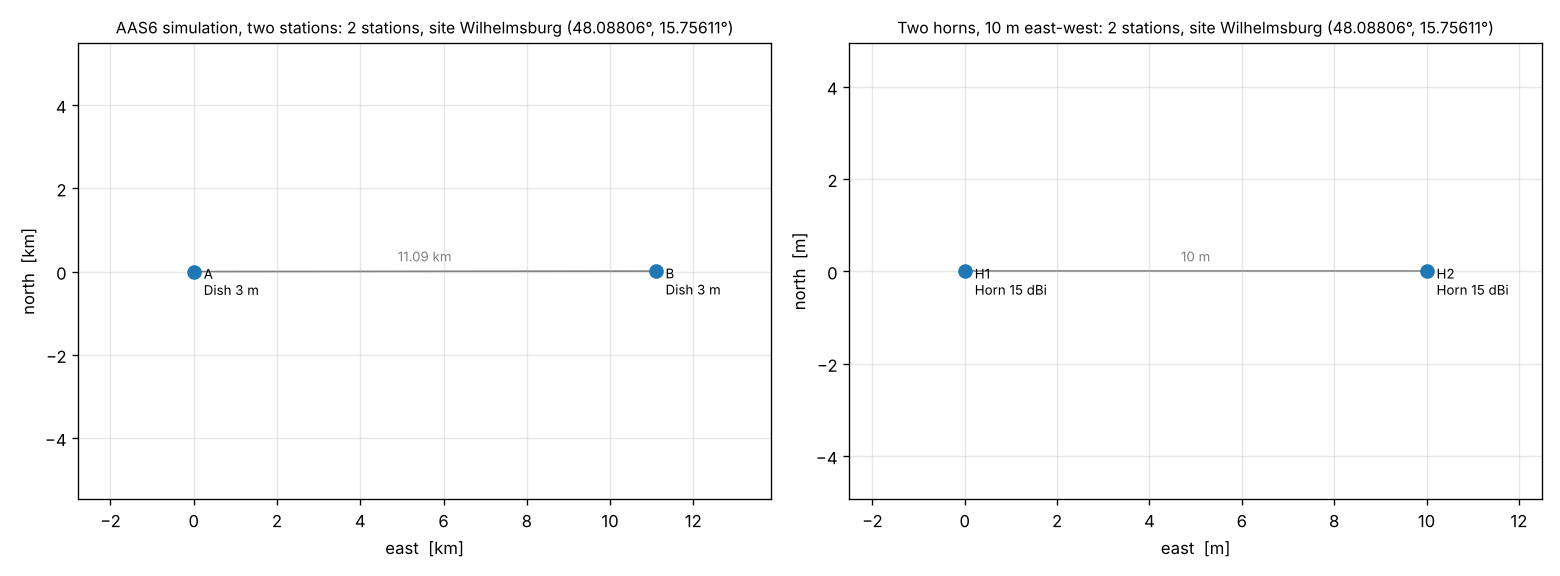
\includegraphics[width=\textwidth]{images/instrument_arrays.png}
  \caption{The configured arrays in the local frame of the site
           Wilhelmsburg (\texttt{plot\_array()}).}
  \label{fig:arrays}
\end{figure}
